\chapter{Introduction}
  \section{Overview}
  Microseconds after the Big Bang, the Universe existed in a state known as
    the Quark Gluon Plasma (QGP).
  In the QGP, quarks and gluons are not in hadronic bondage, forced to 
    the confines of bound states such as protons and neutrons.
  The Large Hadron Collider (LHC) produces QGP in the lab in lead-lead (PbPb)
    collisions.
  The high energies and rates of the collisions at the LHC make it possible 
    to do detailed studies of the QGP. 
  The LHC is producing rare experimental probes such as suppressed jets and 
    heavy quarkonia at an unprecedented rate in heavy ion collisions. 
  As a result of recent LHC studies, physicists now have better constraints on 
    the properties like temperature, viscosity, and energy density of the QGP.

  The detailed studies of PbPb collisions coming out of the LHC 
    experiments require an understanding of the initial state of the ions 
    before they collide.
  Without more knowledge of the initial state, physicists cannot determine 
    which experimental effects are due to the QGP and which effects are 
    inherent to the nuclei themselves. 
  For example, suppression of heavy quarkonia is a signature of the QGP 
    but also appears to occur in deuterium-gold collisions where the QGP is not
    expected to arise \cite{dAuOniaPHENIX}. 
  Another important example is measurement of the viscosity, which depends on 
    the relationship between the observed azimuthal anisotropy and the 
    initial eccentricity of the overlap of the two colliding nuclei. 
  A clean probe of the initial state is needed by physicists to comprehensively 
    understand the QGP.
  Ultra-Peripheral Collisions (UPC) at the LHC provide such a probe.

  The current understanding of heavy ion collisions evolved over the
    last 30 years.
  Relativistic heavy ion collisions were first studied using the 
    Alternating Gradient Synchrotron (AGS) at Brookhaven National Lab (BNL) 
    in Upton, NY, followed by the Super Proton Synchrotron (SPS) at CERN near 
    Geneva, Switzerland. 
  From the numerous AGS and SPS experiments two main observables emerged,
    namely, \JPsi{} suppression and strangeness enhancement \cite{sps}. 
  These results pioneered the search for the QGP. 

  The AGS and SPS experiments were fixed target experiments.
  At AGS the ion isotopes $^{16}$O, $^{28}$Si, and $^{197}$Au beams were 
    collied with fix targets. 
  At SPS the same fix target configuration was used, but the ion isotopes were 
    $^{16}$O, $^{32}$S, and $^{208}$Pb.
  The center of mass energies per nucleon pair for these experiments ranged
    from just below 5 GeV to 20 GeV. 
  The threshold for creating the QGP requires an energy density of 0.15 
    $\sim$ GeV/fm$^{3}$ and a temperature near 170 MeV \cite{qgpThresh}.
  AGS and SPS just barely reached this threshold.
  Though the strangeness enhancement and \JPsi{} suppression 
    signals indicated that there was likely a deconfined state of quarks 
    and gluons created, at the energies of the AGS and SPS this state perished 
      to quickly to study any of its properties. 

  Plans for a colliding beam machine dedicated to heavy ions was first 
    proposed 1983.
  The proposed machine was designed to reach energies of 200 GeV per nucleon.
  At these energies, the QGP would presist long enough, and a that signs of
    a gas of hot quarks and gluons would emerge.
  In the summer of 2000 RHIC began collisions and the four experiments,
    STAR, PHENIX, BRAHMS, and PHOBOS started taking data. 
  With collision energies of 200 GeV per colliding nucleon, the energies 
    at RHIC were a factor of 10 higher than was previously achieved. 
  RHIC experiments confirmed for the first time the presence of a thermalized 
    state of quarks and gluons.
  Contrary to expectations, the state found at RHIC was found to be 
    strongly coupled fluid with nearly no viscosity \cite{}.

  The LHC heavy ion program began collisions in 2010, colliding PbPb at 
    a center of mass energy of 2.76 TeV per nucleon pair. 
  This corresponds to an increase in the colliding energy by an order of 
    magnitude with respect to RHIC. 
  The LHC experiments, ALICE, ATLAS, and CMS have studying the heavy ion 
    collisions since then. 
  In 2013 LHCb joined the LHC heavy ion program. 
  Thanks to the LHC and RHIC physics programs, a new era of precision
    heavy ion measurements is underway. 

  The latest results from the LHC have come from the 2013 proton-lead (pPb)
    run.
  This period of data taking was originally designed to be a control 
    measurement.
  For example, the initial suppression signals observed in dAu collisions at 
    RHIC were believed to be due to non-QGP effects \cite{ }. 
  The azimuthal anisotropy of particles present in PbPb and AuAu at the LHC and 
    RHIC respectively were believed to be signals of flow from the QGP and 
    would not appear in the lower density pp and pPb collisions.
  However, CMS showed evidence of a flow signal in high multiplicity pp events
    in early 2011 \cite{ }. 
  More recently ALICE has shown a structure in two particle correlation 
    measurements, referred to as the double ridge \cite{ }, and CMS and ALICE have both 
    shown an elliptical flow signal present in the pPb data \cite{}.

  The latest data from the pPb and dAu measurements confirm the need to 
    understand the nature of the initial state. 
  UPC events fulfill this need by probing the nucleus through photon 
    interactions.
  By measuring UPC \JPsi{} events, theoretical models of the initial state can 
    be constrained.
  In this thesis, the CMS capability for measuring this process, the 
  description of the analysis, and the comparison between the measured 
    coherent \JPsi{} cross section to theoretical models are given. 

  \section{Significant HI measurments of the QGP}
    The big measurement from RHIC: hadron Raa, elliptic flow
    \begin{figure}[!Hhbt]
      \centering
      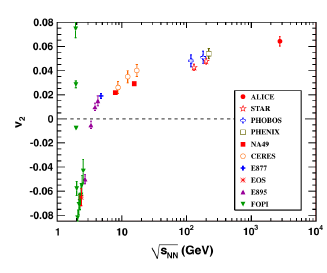
\includegraphics{elipFlow}
      \caption{ $v^{2}$ elliptical flow measurements from SPC to the LHC.}
      \label{fig:elipFlow}
    \end{figure}

     \begin{figure}[!Hhbt]
      \centering
      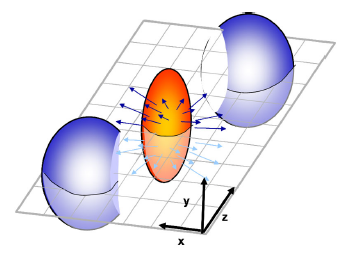
\includegraphics{elipFlowSchem}
      \caption{ Elliptical flow schematic diagram.}
      \label{fig:elipFlowSchem}
    \end{figure}

    \begin{figure}[!Hhbt]
      \centering
      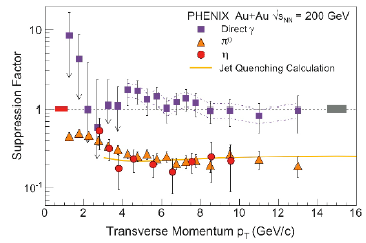
\includegraphics{hadRaaRhic}
      \caption{Hadron R$_{AA}$ from RHIC}
      \label{fig:hadRaaRhic}
    \end{figure}

    \begin{figure}[!Hhbt]
      \centering
      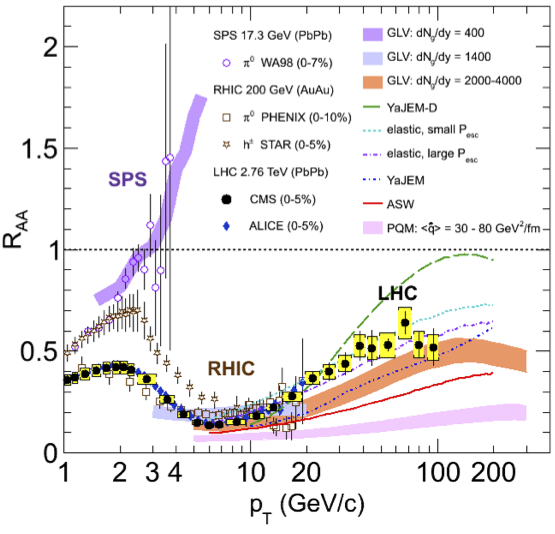
\includegraphics[width=.45\textwidth]{hadRaaLhc}
      \caption{Hadron R$_{AA}$ from the LHC.}
      \label{fig:hadRaaLhc}
    \end{figure}

    \begin{figure}[!Hhbt]
      \centering
      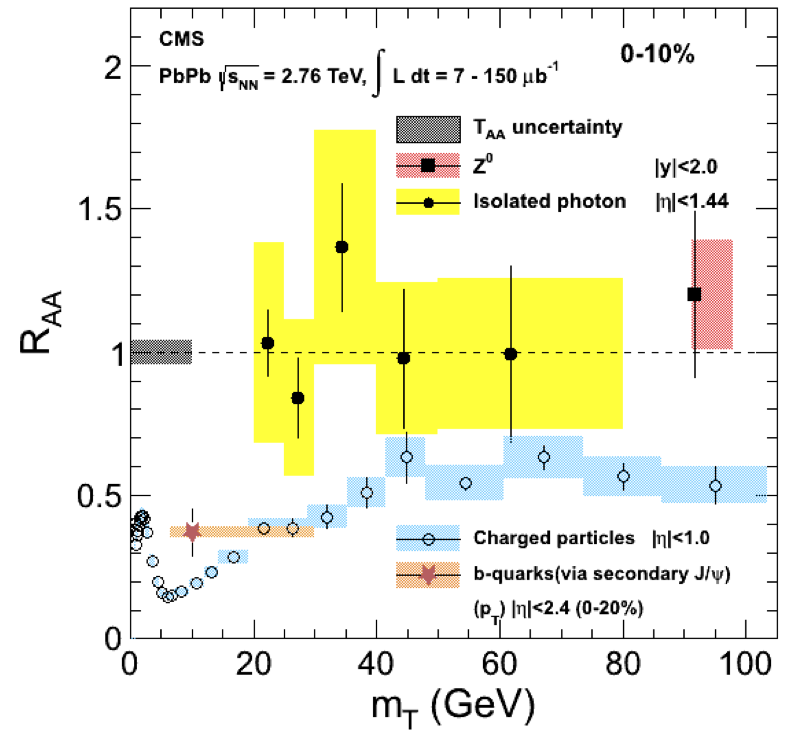
\includegraphics[width=.45\textwidth]{noRaaLhc}
      \caption{R$_{AA}$ for unsuppressed Z bosons and isolated photons.}
      \label{fig:noRaaLhc}
    \end{figure}

  \section{Recent results from HI control measurements}

    \subsection{The HI collision}
      The AGS and SPS created the first signs of a deconfined state, but the 
        nature of the state was uncertain.
      At RHIC the existence of the QGP was confirmed and it's nature found to 
        be hydrodynamic.
      The LHC and RHIC experiments are now looking deeper in the characteristics
        of QGP.
      More precise and sophisticated measurement techniques now require a 
        better understanding of the ions before they collide in order to 
        produce the proper theoretical modeling. 

      Over the course of the experimental evolution the following picture of 
        a heavy ion collision emerged. 
      First, highly contracted ions travel toward each other.
      Second, QGP forms and reaches thermal equilibrium.
      Third, this hot dense state expands hydrodynamically.
      Fifth, Fifth as the collection of quarks and gluons cool, a gas of hot
        hadrons forms and expands.
      Finally, all interactions freeze out and the produced particles stream 
        to the detector. 
